\documentclass[a4paper,11pt]{jsarticle}


% 数式
\usepackage{amsmath,amsfonts}
\usepackage{bm}
% 画像
\usepackage[dvipdfmx]{graphicx}


\begin{document}

\title{ブロック符号の課題}
\author{}
\date{\today}
\maketitle

\section{組織符号に変換}
\begin{equation*}
  \begin{bmatrix}
    0 & 1 & 1 \\
    1 & 1 & 0 \\
    1 & 1 & 1
  \end{bmatrix}
  \begin{bmatrix}
    1 & 0 & 1 & 0 & 1 & 1 \\
    1 & 1 & 1 & 1 & 0 & 1 \\
    0 & 1 & 1 & 0 & 0 & 1
  \end{bmatrix}=
  \begin{bmatrix}
    1 & 0 & 0 & 1 & 0 & 0 \\
    0 & 1 & 0 & 1 & 1 & 0 \\
    0 & 0 & 1 & 1 & 1 & 1
  \end{bmatrix}
\end{equation*}

\section{標準アレイ}
\begin{table}[hbtp]
  \caption{標準アレイ}
  \label{table:data_type}
  \centering
  \begin{tabular}{c|ccccccc}
    000000 & 001111 &	010110 & 011001	& 100100 & 101011 &	110010 & 111101 \\
    \hline
    000001 & 001110 &	010111 & 011000 &	100101 & 101010	& 110011 & 111100 \\
    000010 & 001101	& 010100 & 011011	& 100110 & 101001 & 110000 & 111111 \\
    001000 & 000111	& 011110 & 010001	& 101100 & 100011	& 111010 & 110101 \\
    010000 & 011111	& 000110 & 001001	& 110100 & 111011 & 100010 & 101101 \\
    100000 & 101111	& 110110 & 111001	& 000100 & 001011	& 010010 & 011101 \\
    101000 & 100111 & 111110 & 110001 & 001100 & 000011 & 011010 & 010101 \\
    100001 & 101110	& 110111 & 111000	& 000101 & 001010	& 010011 & 011100
  \end{tabular}
\end{table}

復号結果は以下の通り。

\begin{table}[hbtp]
  \caption{復号結果}
  \label{table:decoded}
  \centering
  \begin{tabular}{|cc|}
    \hline
    受信語 & 復号結果 \\ \hline \hline
    101110 & 001111 \\ \hline
    010101 & 111101 \\ \hline
    110011 & 110010 \\ \hline
  \end{tabular}
\end{table}

\section{(8, 4)組織符号}
\begin{eqnarray*}
  p_0 &= u_1 + u_2 + u_3 \\
  p_1 &= u_0 + u_1 + u_2 \\
  p_2 &= u_0 + u_1 + u_3 \\
  p_3 &= u_0 + u_2 + u_3
\end{eqnarray*}
\subsection{生成行列}
\begin{equation*}
  \begin{bmatrix}
    1 & 0 & 0 & 0 & 0 & 1 & 1 & 1 \\
    0 & 1 & 0 & 0 & 1 & 1 & 1 & 0 \\
    0 & 0 & 1 & 0 & 1 & 1 & 0 & 1 \\
    0 & 0 & 0 & 1 & 1 & 0 & 1 & 1
  \end{bmatrix}
\end{equation*}

\subsection{パリティ検査行列}
\begin{equation*}
  \begin{bmatrix}
    0 & 1 & 1 & 1 & 1 & 0 & 0 & 0 \\
    1 & 1 & 1 & 0 & 0 & 1 & 0 & 0 \\
    1 & 1 & 0 & 1 & 0 & 0 & 1 & 0 \\
    1 & 0 & 1 & 1 & 0 & 0 & 0 & 1
  \end{bmatrix}
\end{equation*}

\subsection{最小ハミング距離}

\begin{table}[hbtp]
  \caption{情報源と符号の対応}
  \label{table:all-code}
  \centering
  \begin{tabular}{|cc|}
    \hline
    情報源 & 符号 \\ \hline \hline
    0000 & 00000000 \\ \hline
    0001 & 00011011 \\ \hline
    0010 & 00101101 \\ \hline
    0011 & 00110110 \\ \hline
    0100 & 01001110 \\ \hline
    0101 & 01010101 \\ \hline
    0110 & 01100011 \\ \hline
    0111 & 01111000 \\ \hline
    1000 & 10000111 \\ \hline
    1001 & 10011100 \\ \hline
    1010 & 10101010 \\ \hline
    1011 & 10110001 \\ \hline
    1100 & 11001001 \\ \hline
    1101 & 11010010 \\ \hline
    1110 & 11100100 \\ \hline
    1111 & 11111111 \\ \hline
  \end{tabular}
\end{table}

0ベクトル以外の符号の最小ハミング重みが4なので、
最小ハミング距離は4である。

\subsection{訂正できる誤りパターン}
訂正できる誤りパターン数は、0誤りを含むと
\begin{equation*}
  2^{n-k}=2^{8-4}=2^4=16
\end{equation*}
である。誤りパターンは表\ref{table:error-pattern}のように選択できる。

\begin{table}[hbtp]
  \caption{訂正できる誤りパターンの一例}
  \label{table:error-pattern}
  \centering
  \begin{tabular}{cccc}
    00000000 & 00000001 & 00000010 & 00000100 \\
    00001000 & 00010000 & 00100000 & 01000000 \\
    10000000 & 00000011 & 00000110 & 00001010 \\
    00010010 & 00100010 & 01000010 & 10000010
  \end{tabular}
\end{table}

\subsection{符号化回路}

% 図はPDFで作りましょう!
\begin{figure}[htbp]
  \begin{center}
  % サイズはそのまま
  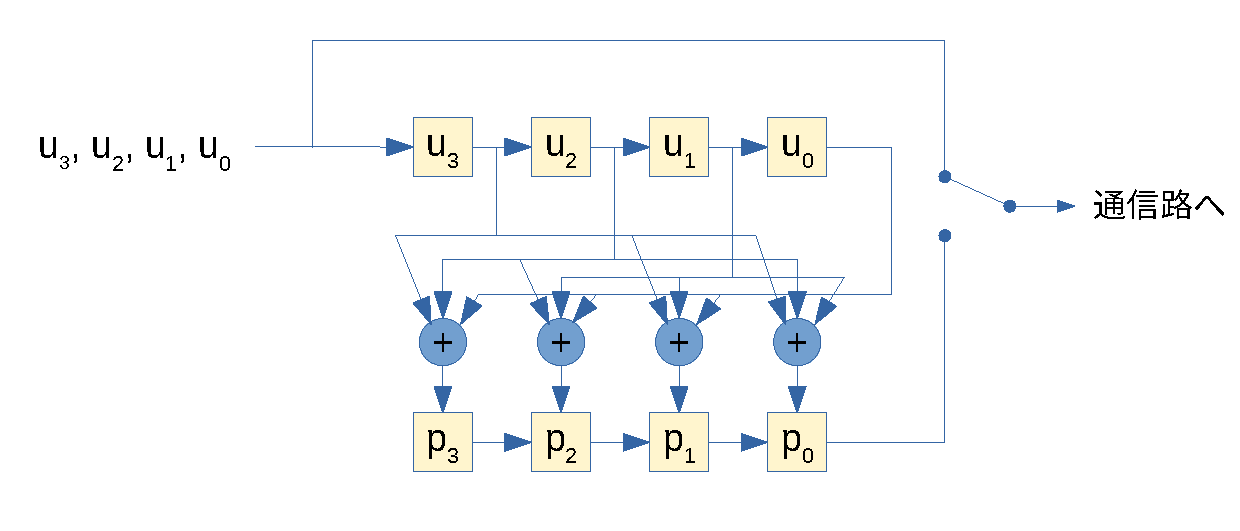
\includegraphics[scale=0.7]{figures/circuit001.pdf}
  \end{center}
  \caption{符号化回路
  \label{fig:pm1}
  }
\end{figure}

\subsection{重み分布と誤りを検出できない確率}
表\ref{table:all-code}より、重み分布は表\ref{table:weight-dist}となる。

\begin{table}[hbtp]
  \caption{重み分布}
  \label{table:weight-dist}
  \centering
  \begin{tabular}{|c|ccc|}
    \hline
    $i$ & 0 & 4 & 8 \\ \hline
    $A_i$ & 1 & 14 & 16 \\ \hline
  \end{tabular}
\end{table}

\end{document}